\begin{figure}[h!]
\centering
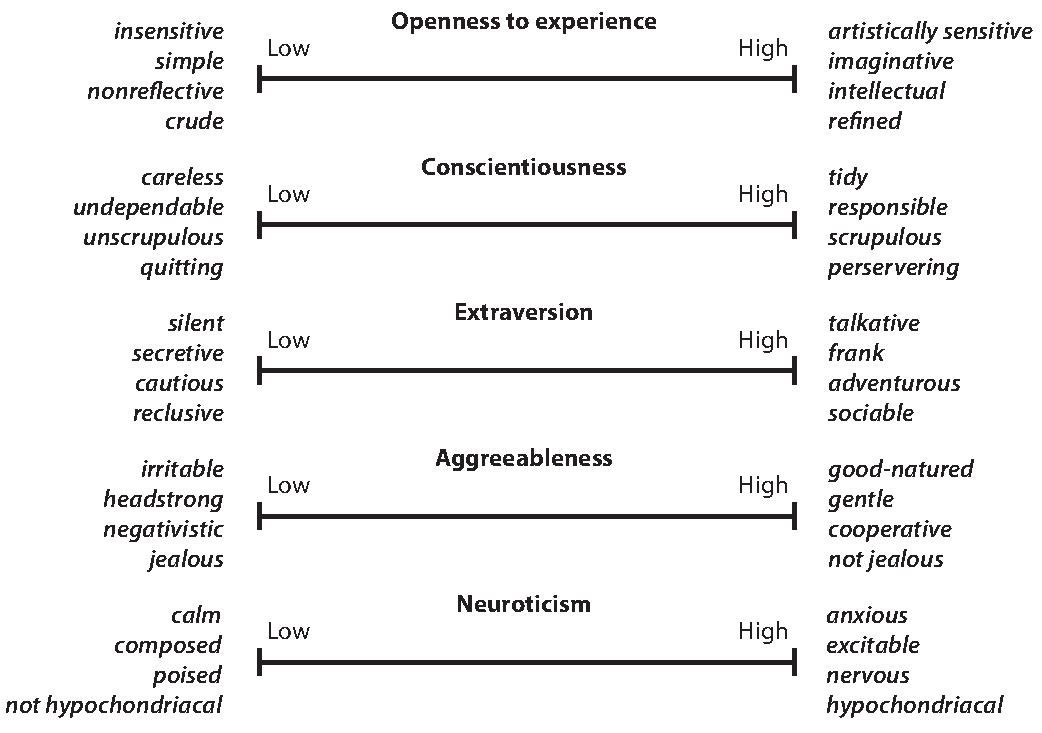
\includegraphics[width=\linewidth]{figures/bigfive}
\caption{\label{fig:bigfive}Visualization of the BFM. Traits are shown in the order 'OCEAN', each constituting a continuous domain between low trait value, associated with adjectives that oppose the name of the trait, and high trait value, associated with adjectives that support the trait name. The model explains an individual's personality as a vector with one score per trait. Scored are typically obtained through a questionnaire inventory.}
\end{figure}

Human efforts to derive a taxonomy for character traits predate our calender. Early efforts include the four \textit{Cardinal Virtues} - prudence, temperance, courage and justice - due to Plato and Aristotle\mcite{Broadie1991-BROEWA}, as well as the four humors - blood, yellow bile, black bile and phlegm - said to have originated in Ancient Egyptian medicine but formalized by Hippocrates\mcite{lloyd1978hippocratic}.
The foundation of the field now known as \textit{trait theory} is, however, not considered rooted in this way thinking. Rather it started in 1884 when Sir Francis Galton established the \textit{lexical hypothesis} which states that any trait that is truly important to humans will become encoded into their language\mcite{galton1949measurement}. Galton reported finding exactly 1000 personality descriptive adjectives in the English language. A similar effort was later made by Gordon Allport and Henry Odbert (1936) using the \textit{Webster's Unabridged Dictionary} (2nd Ed.), which resulted in a 17,953 long list of unique words to describe personality and behavior\mcite{allport1936trait}. The first effort to understand the underlying structure of this vocabulary was taken by Raymond B. Cattell (1943) who applied factor analysis to the covariance structure of words when used to describe individuals in large test groups, and found 16 primary and eight secondary traits\mcite{cattell1945description}. This result was refined by Donald. M. Fiske (1949) who, in an effort to replicate Cattell's result, arrived at a five factor solution\mcite{digman1990personality}. Supported by later research, this is still the prevailing result. It was coined the \textbf{Big Five model}\footnote{Also commonly referred to as the Five Factor model (FFM).} (BFM) by Lewis Goldberg (1981)\mcite{goldberg1981language}, but credit for its invention is typically given to Fiske\mcite{fiskepersonality}. The model is shown in Figure \ref{fig:bigfive}. It offers five high-level personality traits: \textit{openness to experience} (\OPE), \textit{conscientiousness} (\CON), \textit{extraversion} (\EXT), \textit{aggreeableness} (\AGR) and \textit{neuroticism} (\NEU)\mcite{920817074619920601}, which are typically recalled using acronyms OCEAN or CANOE. Traits in the BFM is typically measures using a questionnaire inventory such as the Big Five Inventory or the IPIP100 Inventory which relies on honest self-report by the subject\mcite{IPIPwebsite}. Rather than reducing the rich tapestry of the human psychology to mere five traits, the model seeks to provide a compelling framework for organizing the enormous variety of psychological differences characterizing humans. It assumes a hierarchical view of psychological traits, where the Big Five traits (BFT) are independent roots that each branch into many facets and subfacets.

\subparagraph*{Criticism} The BFM is widely accepted among a substantial number of researchers, by some even considered a universally valid structure that transcends culture and language\mcite{bouchard2001genes, mccrae1997personality}. Unsurprisingly this particular viewpoint is not unchallenged. Recent findings have shown the BFM to only explain variance in a subset of traits (\CON, \EXT, \NEU) for indigenous societies\mcite{gurven2013universal}, which resonates with the finding that \textit{humility} emerges as a trait when studying populations in Asia (as captured by the HEXACO model, see below). Furthermore the lexical hypothesis has been argued to have the two following problems: (1) since language itself is not developed by experts, the inherent ambiguity of words causes any model based on language sampling to, at best, reflect only a lay perceptions of the traits\mcite{cervone2007a, westen1996model}, and (2) words can't accurately capture the spectrum of personality because some very important traits are tacit\mcite{argyle1973a}.

\subparagraph*{Limitations} It has been shown that the BFM only captures up to 56\% of a persons personality spectrum\mcite{boyle1995measurement}. This is very important knowledge to have when using the BFM in any study that attempts to make general statements about personality. In the current undertaking, it too must be respected that certain fine-grained aspect of personality won't be captured and therefore shouldn't be speculated about. Unlike the Eysenck model (presented below) the BFM doesn't for example capture personality variance due to \textit{psychotism}. It thus stands to reason that any strategies inferred from a dataset of BFTs cannot possibly be purely psychopathy, although it is in fact a proven evolutionarily stable strategy (ESS, see Section \ref{subsubsec:individualDifferencesAndPersonality})\mcite{workman2014evolutionary}.

\subparagraph*{Alternative models} While the BFM is the most commonly used system for measuring personality traits, it is not the only one. The HEXACO model of personality structure is another widely accepted model which has deeper roots in European and Asian languages. Using factor analysis it finds six traits, where five are similar to those in the BFM, and one is related to honesty and humility\mcite{ashton2004six}. Another important model is Cattell's 16PF questionnaire which measures personality on 16 out of his original 24 personality dimensions\mcite{cattell2008sixteen}. Finally, the Eysenck personality questionnaire reduces personality into mere three traits: \textit{psychoticism},	\textit{extraversion} and \textit{neuroticism}. In this model psychoticism captures the aggressive and more extreme nuances of neuroticism. Rather than capturing a wide spectrum of personality the Eysenck model aims only at capturing personality variance associated with temperament.